\section{Auswertung}
\label{sec:Auswertung}

\begin{figure}
  \centering
  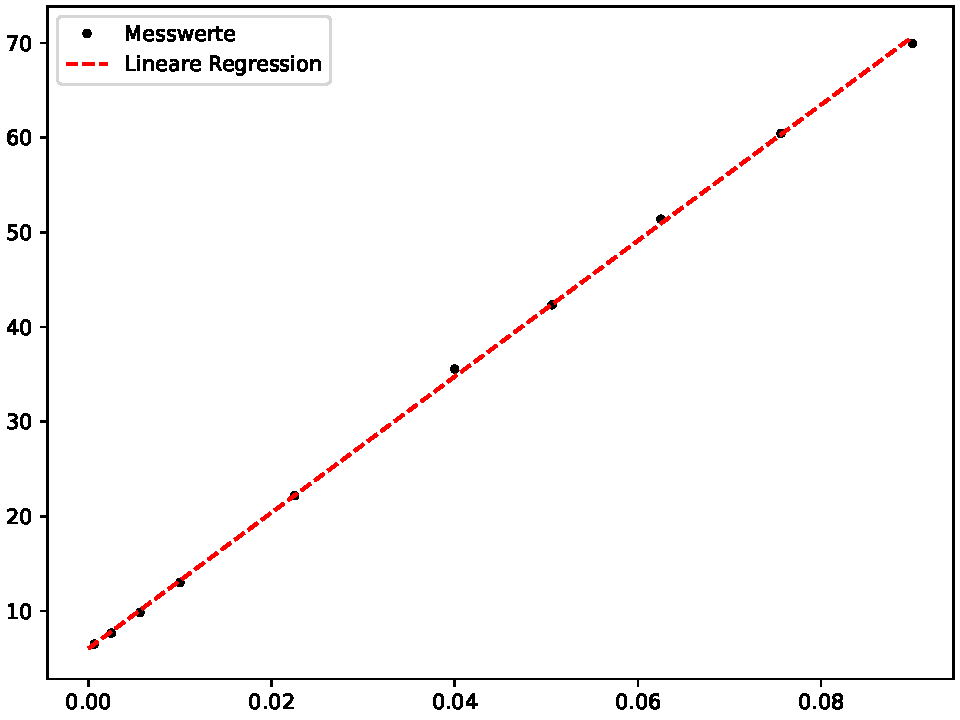
\includegraphics{plot.pdf}
  \caption{Plot.}
  \label{fig:plot}
\end{figure}

\begin{table}
  \centering
  \caption{Eine Beispieltabelle mit Messdaten.}
  \label{tab:tabelle}
  \sisetup{table-format=1.1, per-mode=reciprocal}
  \begin{tblr}{
      colspec = {S[table-format=3.0] S[table-format=2.1] S},
      row{1} = {guard, mode=math},
      vline{4} = {2}{-}{text=\clap{$\pm$}},
    }
    \toprule
    U \mathbin{/} \unit{\volt} & I \mathbin{/} \unit{\micro\ampere} & \SetCell[c=2]{c} N \mathbin{/} \unit{\per\second} & \\
    \midrule
    360 & 0.1 & 98.3 & 0.9 \\
    400 & 0.2 & 99.8 & 1.0 \\
    420 & 0.2 & 99.1 & 0.9 \\
    \bottomrule
  \end{tblr}
\end{table}

Siehe \autoref{fig:plot} und \autoref{tab:tabelle}!
